\documentclass[UKenglish]{uioexam}
\usepackage{amsmath}
\usepackage{amssymb}
\usepackage{tabularx}

\usepackage{tabularx}
\usepackage{url}
\usepackage{hyperref}
\hypersetup{
    colorlinks=true,
    linkcolor=blue,
    filecolor=magenta,      
    urlcolor=blue,
    pdftitle={Overleaf Example},
    pdfpagemode=FullScreen,
    }
\newcommand{\answerbox}{\fbox{\phantom{M}}}
\usepackage{setspace}
\usepackage{minted}
\usepackage{graphicx}
\usepackage[T1]{fontenc}
\usepackage[french]{babel,textcomp}
\usepackage{multicol}
\dato{7 décembre 2023, 08h-09h}
\emne{\textsc{}}{}
\tid{}{}
\usepackage{eso-pic}


\begin{document}
    \AddToShipoutPictureFG*{
    \AtPageUpperLeft{\put(-50,-50){\makebox[\paperwidth][r]{\huge/20}}}  
    }%
\onehalfspacing
\section[REN]{\small(4 points)}
Dans la phrase suivante, soulignez toutes les entités nommées :

\textit{Emmanuel Macron, né le 21 décembre 1977 à Amiens, est président de la France.}

\end{choicelist}

\section[Regex]{\small(1 point)}
Parmi les options ci-dessous, choisissez celle(s) qui correspond(ent) à (aux) expression(s) régulière(s) valide(s) :
\begin{choicelist}[]
    \choice
    \texttt{\^{}jour}
    
    \choice
    \texttt{[[\^{}jour}

    \choice
    \texttt{[a-zA-Z0-9\_])}
    
    \choice
    \texttt{[a-zA-Z0-9\_]}


\end{choicelist}

\section[Méthodes/Segnentation]{\small(1 point)}
Comment s'appelle l'étape initiale d'une chaîne de traitement d'OCR ?
\begin{choicelist}[]
    \choice
    exportation

    \choice
    prédiction

    \choice
    transcription

    \choice
    segmentation
\end{choicelist}

\section[Transkribus]{\small(1 point)}
Remplissez le blanc avec le mot approprié :

Transkribus est une plateforme de la \makebox[5cm]{\hrulefill} automatique des textes.

\section[Cartographie]{\small(2 points)}
L'illustration suivante représente un exemple de :

(plusieurs réponses possibles)
\begin{choicelist}[]
    \choice
    l'annotation des entités nommées suivant le format \textsc{BIO}

    \choice
    la cartographie des entités nommées

    \choice
    la campagne d'évaluation de la reconnaissance d'entités nommées

    \choice
    la désambiguïsation des entités nommées
    
\end{choicelist}

\begin{figure}[h!]
    \centering
    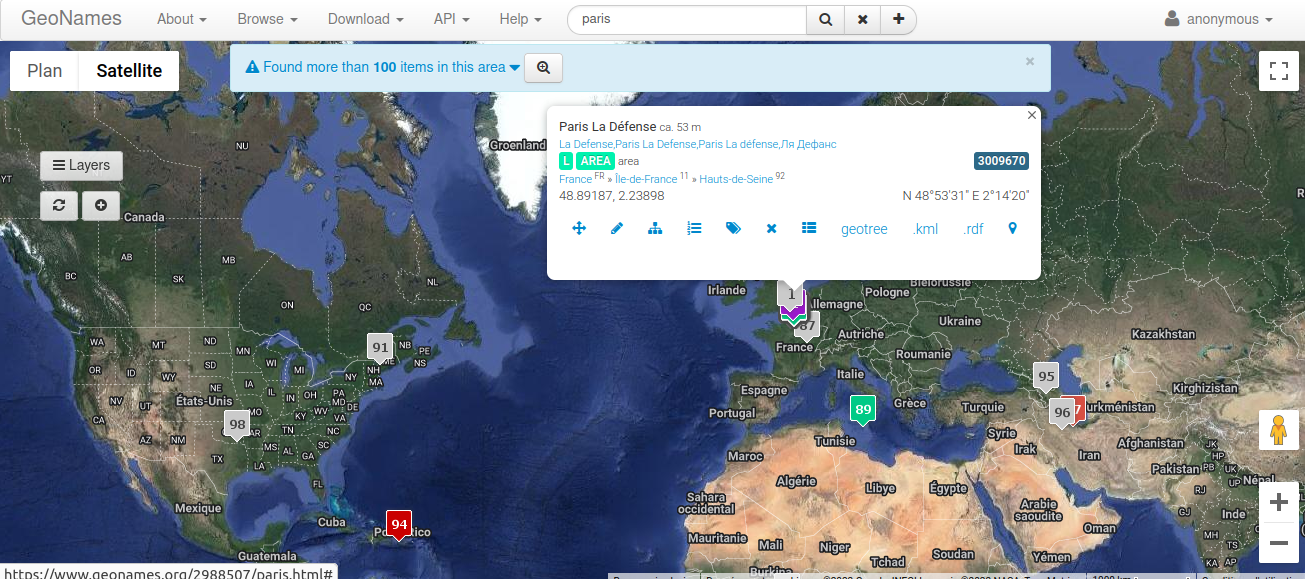
\includegraphics[width=1\textwidth]{img/geonames.png}
    % \caption{a nice plot}
    \label{fig:mesh1}
\end{figure}



\section[Regex]{\small(1 point)}
Quel est l'intérêt d'utilisation des expressions régulières ?\\~\\
\framebox(390,50){}


\section[Regex · Export OCR / HTR]{\small(2 points)}
Répondez par \textsc{Vrai} (\textsc{V}) ou \textsc{Faux} (\textsc{F}) aux phrases suivantes :\\
\newcounter{abc}
\renewcommand{\theabc}{\stepcounter{abc}\alph{abc}}
\newcommand{\answerbox}{\fbox{\phantom{M}}}
\begin{document}
\def\arraystretch{2}% increase vertical spacing
\noindent\begin{tabularx}{\textwidth}{cXcc}
 & & V & F\\
(\theabc) & L'approche à base de règles pour effectuer certaines tâches de TAL nécessite un entraînement d'un modèle.  & \answerbox & \answerbox\\
(\theabc) & Généralement, les logiciels d'OCR / HTR permettent d'exporter des transcriptions dans différents formats. & \answerbox & \answerbox
\end{tabularx}

\section[Regex_pratique]{\small(2 points)}

Étant donné la phrase \textit{Je suis en train de réviser pour mon 2\textsuperscript{ème} partiel}, 

formulez les regex qui permettent de capturer les mots suivants :

\begin{enumerate}
\item \textit{2\textsuperscript{ème}} \makebox[3cm]{\hrulefill}
\item \textit{Je} \makebox[3cm]{\hrulefill}
\end{enumerate}

Pour tester vos regex, vous pouvez utiliser un site dédié comme, p. ex. \url{https://regex101.com/}. 

\textbf{Attention} : les réponses qui utilisent uniquement les caractères littéraux \textit{2\textsuperscript{ème}} et \textit{Je} ne sont pas acceptées.

\section[Voyant_Tools]{\small(3 points)\label{voyant}}
\begin{enumerate}
\item Chargez le corpus \href{https://icampus.univ-paris3.fr/mod/resource/view.php?id=639612}{\textit{Le tour du monde en quatre-vingts jours}} (utilisé lors de la séance du 23 novembre 2023, \og{}Reconnaissance d'entités nommées\fg{}) dans \href{https://voyant-tools.org/}{Voyant Tools} depuis votre ordinateur ;

\item Combien de \textit{tokens} et de \textit{types} ce corpus contient-il ?  

Tokens : \makebox[2cm]{\hrulefill} 

Types : \makebox[2cm]{\hrulefill}
\item Quelle est la fréquence absolue du mot \texttt{fogg} ? \makebox[2cm]{\hrulefill}
\end{enumerate}

\section[Tanagra]{\small(3 points)}

\begin{enumerate}
\item Dirigez-vous vers la page de l'outil \href{https://obtic.sorbonne-universite.fr/tanagra/map}{Tanagra}.

Sélectionnez \texttt{French\_lg} comme modèle de reconnaissance d'entités nommées et chargez le même corpus que dans la question \ref{voyant}. 

\item Parmi les entités nommées récupérées par Tanagra, en trouvez-vous une localisée en Espagne ? Si oui, laquelle ? \\~\\\framebox(390,50){}
\end{enumerate}

\end{document}

